%% Relatório de Estágio Curricular
%% Danilo Godofredo de Mattos
%% Engenharia de Computação - UNIFEI
%% Baseado no modelo abntex2

\documentclass[
	12pt,
	oneside,
	a4paper,
	brazil,
	sumario=tradicional
]{abntex2}

% Pacotes básicos
\usepackage[T1]{fontenc}
\usepackage[utf8]{inputenc}
\usepackage{lmodern}
\usepackage{indentfirst}
\usepackage{color}
\usepackage{graphicx}
\usepackage{microtype}
\usepackage{float}
\usepackage{listings}
\usepackage{xcolor}
\usepackage{tikz}
\usetikzlibrary{shapes.geometric, arrows, positioning, fit, backgrounds}

% Pacotes de citações
\usepackage[brazilian,hyperpageref]{backref}
\usepackage[alf]{abntex2cite}

% Configuração do listings para código
\definecolor{codegreen}{rgb}{0,0.6,0}
\definecolor{codegray}{rgb}{0.5,0.5,0.5}
\definecolor{codepurple}{rgb}{0.58,0,0.82}
\definecolor{backcolour}{rgb}{0.95,0.95,0.92}

\lstdefinestyle{mystyle}{
    backgroundcolor=\color{backcolour},
    commentstyle=\color{codegreen},
    keywordstyle=\color{magenta},
    numberstyle=\tiny\color{codegray},
    stringstyle=\color{codepurple},
    basicstyle=\ttfamily\footnotesize,
    breakatwhitespace=false,
    breaklines=true,
    captionpos=b,
    keepspaces=true,
    numbers=left,
    numbersep=5pt,
    showspaces=false,
    showstringspaces=false,
    showtabs=false,
    tabsize=2
}
\lstset{style=mystyle}

% Informações do documento
\titulo{Relatório Final de Estágio Curricular}
\autor{Danilo Godofredo de Mattos}
\local{Brasil}
\data{Novembro de 2025}
\orientador{Prof. Dr. Ramon Maia Borges}
\instituicao{%
  Universidade Federal de Itajubá -- UNIFEI
  \par
  Instituto de Engenharia de Sistemas e Tecnologia da Informação
  \par
  Engenharia da Computação}
\tipotrabalho{Relatório de Estágio}

% Configurações de aparência do PDF final
\makeatletter
\hypersetup{
     	pdftitle={\@title},
     	pdfauthor={\@author},
     	pdfsubject={Relatório de Estágio},
	    pdfcreator={LaTeX with abnTeX2},
		pdfkeywords={estágio}{desenvolvimento de software}{web scraping}{startup},
		colorlinks=true,
    	linkcolor=blue,
    	citecolor=blue,
    	filecolor=magenta,
		urlcolor=blue,
		bookmarksdepth=4
}
\makeatother

% Espaçamentos entre linhas e parágrafos
\setlength{\parindent}{1.3cm}
\setlength{\parskip}{0.2cm}

% Início do documento
\begin{document}

\selectlanguage{brazil}

\frenchspacing

% Capa
\imprimircapa

% Folha de rosto
\imprimirfolhaderosto*

% Lista de ilustrações
\pdfbookmark[0]{\listfigurename}{lof}
\listoffigures*
\cleardoublepage

% Sumário
\pdfbookmark[0]{\contentsname}{toc}
\tableofcontents*
\cleardoublepage

% Elementos textuais
\textual

% ----------------------------------------------------------
% CAPÍTULO 1: Introdução
% ----------------------------------------------------------
\chapter{Introdução}

Este relatório contém as principais atividades desenvolvidas pelo aluno Danilo Godofredo de Mattos, estudante de Engenharia de Computação na Universidade Federal de Itajubá, durante o estágio obrigatório realizado na área de desenvolvimento de sistemas da empresa Simple Juris, que ocorreu a partir de 7 de Janeiro de 2024 até 7 de Janeiro de 2025.

O aluno trabalhou como um dos fundadores da startup Simple Juris, atuando como principal desenvolvedor fullstack. Desse modo, participou ativamente do desenvolvimento da plataforma web que automatiza o acompanhamento de processos judiciais para advogados. A oportunidade de trabalhar em uma startup trouxe desafios diferentes dos encontrados em estágios tradicionais, exigindo decisões sobre arquitetura, escolha de tecnologias e resolução de problemas de infraestrutura em produção.

Nos capítulos seguintes, são apresentadas informações sobre a empresa, os dados formais do estágio e, em maior detalhe, as atividades técnicas desenvolvidas ao longo desse período.

% ----------------------------------------------------------
% CAPÍTULO 2: A Empresa
% ----------------------------------------------------------
\chapter{A Empresa}

\section{Dados da Empresa}

\noindent\textbf{Nome:} Simple Juris

\noindent\textbf{Razão Social:} Simple Juris Software Jurídico LTDA

\noindent\textbf{CNPJ:} 37.896.350/0001-98

\noindent\textbf{Endereço:} Avenida BPS, 1303, SALA 30 PCE, Pinheirinho, Itajubá - MG, CEP: 37.500-903

\noindent\textbf{Ramo de Atividades:} Desenvolvimento de Software

\noindent\textbf{Tipo de Empresa:} Privada

\section{Histórico e Área de Atuação}

A Simple Juris é uma startup fundada na Universidade Federal de Itajubá (UNIFEI) em agosto de 2018, incubada no Parque Científico e Tecnológico da instituição. O estagiário, em conjunto com outros estudantes do curso de Engenharia de Computação, iniciou o projeto após identificar uma demanda recorrente entre advogados: a necessidade de verificar diariamente dezenas de processos nos portais de tribunais para acompanhar as movimentações processuais.

Um advogado com cem processos ativos necessitaria, em tese, acessar o sistema do tribunal cem vezes por dia para garantir que nenhum prazo fosse perdido. Na prática, essa verificação manual torna-se inviável, e movimentações relevantes frequentemente passam despercebidas. A proposta da Simple Juris consiste em automatizar esse acompanhamento por meio de técnicas de web scraping, notificando o profissional por e-mail somente quando alterações significativas são detectadas.

Além do monitoramento automatizado, a plataforma mantém o histórico completo de movimentações e disponibiliza os diários oficiais dos tribunais em formato pesquisável.

\section{Responsável pelo Estágio}

\noindent\textbf{Nome:} Misael Cézar Gomes de Souza

\noindent\textbf{Cargo:} Sócio e Gerente de Produto

\noindent\textbf{Formação:} Engenharia de Computação - UNIFEI

\noindent\textbf{E-mail:} misael@simplejuris.com

\noindent\textbf{Telefone:} (12) 98130-1884

% ----------------------------------------------------------
% CAPÍTULO 3: O Estágio
% ----------------------------------------------------------
\chapter{O Estágio}

\section{Dados do Estagiário}

\noindent\textbf{Nome:} Danilo Godofredo de Mattos

\noindent\textbf{Matrícula:} 2018009986

\noindent\textbf{Curso:} Engenharia de Computação

\noindent\textbf{Instituição:} Universidade Federal de Itajubá

\noindent\textbf{Ano de Ingresso:} 2018

\noindent\textbf{Endereço:} Rua Domingos Freire, 44, Apto 605, Todos Santos, Rio de Janeiro - RJ

\noindent\textbf{E-mail:} danilo@simplejuris.com

\noindent\textbf{Telefone:} (21) 98136-6797

\section{Informações do Estágio}

\noindent\textbf{Data de Início:} 7 de Janeiro de 2024

\noindent\textbf{Data de Término:} 7 de Janeiro de 2025

\noindent\textbf{Carga Horária Total:} 1.040 horas (20 horas semanais)

\noindent\textbf{Departamento:} Desenvolvimento de Software

\noindent\textbf{Função:} Desenvolvedor Full Stack

\section{Objetivo do Estágio}

O objetivo do estágio foi proporcionar ao aluno a oportunidade de aplicar os conhecimentos adquiridos ao longo do curso de Engenharia de Computação no desenvolvimento de um produto de software em ambiente profissional. Na Simple Juris, o estagiário pôde aprofundar seus conhecimentos em desenvolvimento web, arquitetura de sistemas distribuídos, técnicas de web scraping e infraestrutura em nuvem.

Por atuar como um dos fundadores da empresa, o estagiário dispôs de maior autonomia em comparação a estágios convencionais. Essa posição implicou liberdade para tomar decisões sobre tecnologias e arquitetura do sistema, mas também responsabilidade direta pela resolução de problemas em ambiente de produção.

% ----------------------------------------------------------
% CAPÍTULO 4: Atividades Desenvolvidas
% ----------------------------------------------------------
\chapter{Atividades Desenvolvidas}

Este capítulo descreve as principais atividades técnicas realizadas pelo estagiário durante o período de estágio, desde a definição inicial da arquitetura até a configuração do ambiente de produção.

\section{Definição da Arquitetura do Sistema}

Como principal desenvolvedor fullstack da empresa no momento, o aluno foi responsável por definir a stack de tecnologias a ser utilizada. A decisão levou em conta o conhecimento prévio da equipe, os custos de infraestrutura e a capacidade da arquitetura de suportar o crescimento da base de usuários.

\subsection{Escolha das Tecnologias}

Após avaliar as alternativas disponíveis, o estagiário definiu a seguinte combinação:

\begin{itemize}
    \item \textbf{Backend:} Node.js \cite{nodejs_docs} com Express \cite{express_docs}. A escolha foi motivada pela experiência prévia da equipe com JavaScript e pela possibilidade de utilizar a mesma linguagem no frontend e backend.

    \item \textbf{Frontend:} React \cite{react_docs} para a interface web. A abordagem baseada em componentes facilitou a organização do código conforme o projeto crescia.

    \item \textbf{Banco de Dados:} PostgreSQL \cite{postgresql_docs}. A equipe necessitava de um banco relacional confiável, e o suporte nativo a JSON auxiliou no armazenamento de dados semi-estruturados vindos dos tribunais.

    \item \textbf{Web Scraping:} Foi utilizado Axios \cite{axios_docs} para realizar as requisições HTTP e Cheerio \cite{cheerio_docs} para extrair dados do HTML. Para páginas que dependiam de JavaScript, recorreu-se ao Puppeteer \cite{puppeteer_docs}.

    \item \textbf{Armazenamento:} AWS S3 \cite{aws_s3_docs} para armazenar os PDFs dos diários oficiais. O custo é baixo e elimina preocupações com espaço em disco.

    \item \textbf{Infraestrutura:} Docker \cite{docker_docs} para manter os ambientes consistentes, rodando em uma VPS da DigitalOcean \cite{digitalocean_docs}.
\end{itemize}

\subsection{Diagrama de Arquitetura}

A arquitetura do sistema foi organizada conforme ilustrado na Figura \ref{fig:arquitetura}.

\begin{figure}[htb]
	\caption{\label{fig:arquitetura}Arquitetura geral do sistema Simple Juris}
	\begin{center}
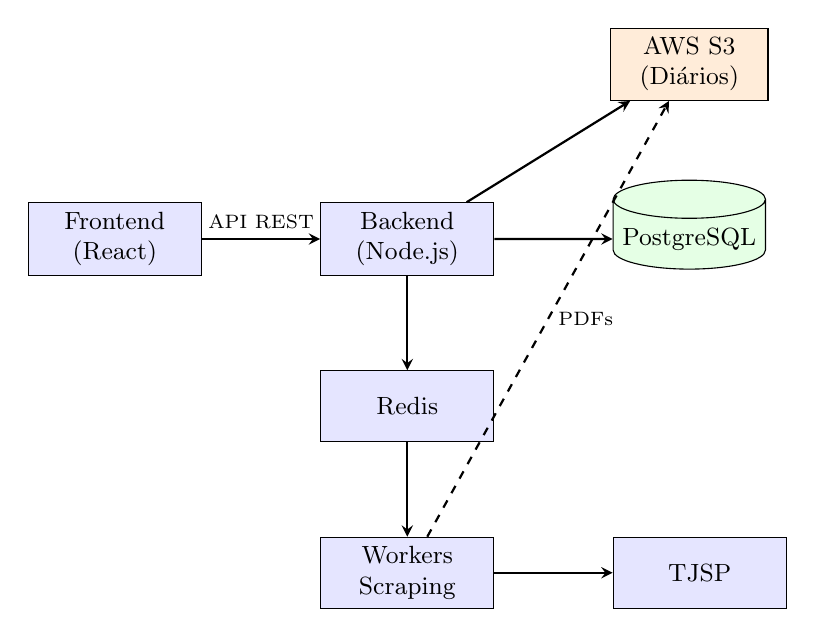
\begin{tikzpicture}[
    node distance=1.2cm,
    box/.style={rectangle, draw, minimum width=2.2cm, minimum height=0.9cm, align=center, fill=blue!10, font=\small},
    db/.style={cylinder, draw, shape border rotate=90, aspect=0.25, minimum height=1cm, minimum width=1.3cm, fill=green!10, font=\small},
    cloud/.style={rectangle, draw, minimum width=2cm, minimum height=0.9cm, align=center, fill=orange!15, font=\small},
    arrow/.style={->, >=stealth, thick}
]

\node[box] (frontend) {Frontend\\(React)};
\node[box, right=1.5cm of frontend] (backend) {Backend\\(Node.js)};
\node[db, right=1.5cm of backend] (db) {PostgreSQL};
\node[cloud, above=1cm of db] (s3) {AWS S3\\(Diários)};
\node[box, below=1.2cm of backend] (redis) {Redis};
\node[box, below=1.2cm of redis] (workers) {Workers\\Scraping};
\node[box, right=1.5cm of workers] (scraper) {TJSP};

\draw[arrow] (frontend) -- node[above, font=\scriptsize] {API REST} (backend);
\draw[arrow] (backend) -- (db);
\draw[arrow] (backend) -- (s3);
\draw[arrow] (backend) -- (redis);
\draw[arrow] (redis) -- (workers);
\draw[arrow] (workers) -- (scraper);
\draw[arrow, dashed] (workers) -- node[right, font=\scriptsize] {PDFs} (s3);

\end{tikzpicture}
	\end{center}
	\legend{Fonte: Elaboração Própria}
\end{figure}

\section{Desenvolvimento do Backend}

O desenvolvimento do backend consumiu a maior parte do tempo de estágio. Esse componente é central na aplicação, sendo responsável por receber as requisições do frontend, gerenciar a autenticação dos usuários, coordenar os workers de scraping e processar os dados antes de persistí-los no banco.

A principal complexidade residia na orquestração assíncrona dessas operações. Considerando que um advogado pode possuir centenas de processos e que cada sincronização dispara dezenas de requisições ao tribunal, realizar essas operações de forma eficiente, sem comprometer a disponibilidade do servidor e respeitando os limites impostos pelo site do tribunal, constituiu um dos maiores desafios técnicos enfrentados.

\subsection{Modelagem do Banco de Dados}

A modelagem do banco de dados exigiu compreender bem o domínio jurídico. O aluno conversou com advogados para entender como eles organizavam mentalmente seus processos e quais informações eram mais importantes no dia a dia.

O modelo final ficou com as seguintes entidades principais:

\begin{itemize}
    \item \textbf{Advogado:} Além dos dados cadastrais, guarda as credenciais criptografadas de acesso a cada tribunal. Um advogado pode ter credenciais em múltiplos tribunais.

    \item \textbf{Tribunal:} Contém configurações específicas de cada tribunal suportado, como URL base, formato de autenticação e intervalos permitidos entre requisições.

    \item \textbf{Processo:} Armazena o número unificado (CNJ), classe processual, vara, partes envolvidas e status atual. A relação com o advogado é de muitos-para-muitos, já que um processo pode ter vários advogados e vice-versa.

    \item \textbf{Movimentação:} Cada registro representa uma publicação ou andamento do processo, com data, descrição e hash do conteúdo para detectar duplicatas.

    \item \textbf{Notificação:} Controla quais movimentações já foram enviadas para cada advogado, evitando notificações duplicadas e permitindo reenvios quando necessário.
\end{itemize}

Foram utilizados índices compostos nas colunas mais consultadas (número do processo + tribunal, advogado + data da movimentação) para manter as queries rápidas mesmo com milhões de registros.

\subsection{Implementação da API REST}

A API conecta o frontend ao banco de dados e dispara as tarefas de scraping. Os principais endpoints são:

\begin{itemize}
    \item \texttt{POST /api/auth/register/} - Cadastro de novo advogado
    \item \texttt{POST /api/auth/login/} - Autenticação via JWT \cite{jwt_docs}
    \item \texttt{GET /api/processos/} - Lista processos do advogado
    \item \texttt{GET /api/processos/\{id\}/movimentacoes/} - Movimentações de um processo
    \item \texttt{POST /api/processos/sincronizar/} - Dispara sincronização manual
\end{itemize}

\subsection{Sistema de Tarefas Assíncronas}

O processo de scraping de um tribunal pode demandar vários minutos para ser concluído, tornando inviável sua execução no contexto de uma requisição HTTP convencional. Para contornar essa limitação, o estagiário implementou um sistema de processamento assíncrono utilizando o Bull \cite{bull_docs}, uma biblioteca de filas baseada em Redis \cite{redis_docs}. Nessa arquitetura, quando um advogado solicita uma sincronização, a API apenas registra a tarefa na fila e retorna uma resposta imediata ao cliente. Um worker dedicado, executando em processo separado, consome as tarefas da fila e realiza as operações de scraping de forma assíncrona.

\section{Desenvolvimento do Sistema de Web Scraping}

O desenvolvimento do sistema de web scraping representou um dos maiores desafios técnicos do projeto. A extração automatizada de dados dos portais de tribunais apresenta complexidades inerentes: esses sistemas não foram projetados para acesso programático, não disponibilizam APIs públicas, sofrem alterações de layout sem aviso prévio e frequentemente implementam mecanismos de bloqueio contra acessos automatizados.

\subsection{Análise e Implementação}

Previamente à implementação do código, o estagiário dedicou tempo significativo à análise detalhada do portal do TJSP, estudando o mecanismo de autenticação, a estrutura de navegação até os dados processuais e as requisições HTTP realizadas internamente pelo navegador. Essa fase de análise mostrou-se essencial para compreender quais comportamentos deveriam ser simulados pelo sistema.

O scraper foi organizado em classes, com uma classe base que define a interface e classes específicas para cada tribunal:

\begin{lstlisting}[language=JavaScript, caption=Estrutura básica do scraper]
class BaseTribunalScraper {
    constructor(advogado) {
        this.advogado = advogado;
        this.cookies = {};
    }

    async autenticar() {
        throw new Error('Not implemented');
    }

    async buscarProcessos() {
        throw new Error('Not implemented');
    }

    async buscarMovimentacoes(processo) {
        throw new Error('Not implemented');
    }
}
\end{lstlisting}

\subsection{Tratamento de Erros}

Sistemas de web scraping estão sujeitos a uma variedade de falhas: alterações na estrutura das páginas do tribunal, instabilidades de conexão, indisponibilidade temporária dos servidores externos, entre outras. Para garantir a robustez do sistema, o estagiário implementou um mecanismo de retry automático com backoff exponencial, no qual o intervalo entre tentativas aumenta progressivamente. Além disso, foram desenvolvidos logs detalhados para facilitar a depuração posterior, alertas automáticos no Slack para falhas recorrentes, e um sistema de salvamento parcial que preserva os dados já coletados em caso de interrupção durante o processo.

\section{Desenvolvimento do Frontend}

A interface web foi desenvolvida utilizando React \cite{react_docs}, com componentes funcionais e hooks como padrão de implementação. O estagiário organizou a estrutura do código em camadas distintas: componentes de layout (cabeçalho, barra lateral), formulários reutilizáveis, componentes específicos do domínio jurídico (cards de resumo de processos, timeline de movimentações) e as páginas que compõem a aplicação.

O gerenciamento do estado global da aplicação foi implementado com Redux Toolkit \cite{redux_docs}, que oferece uma API mais simplificada em comparação ao Redux tradicional, reduzindo a quantidade de código boilerplate necessário. A comunicação com o backend foi realizada através da biblioteca Axios \cite{axios_docs}, que facilita o tratamento de requisições HTTP e interceptação de erros.

\section{Configuração do Ambiente de Produção}

A implantação do sistema em ambiente de produção foi realizada em uma VPS (Virtual Private Server) da DigitalOcean \cite{digitalocean_docs}, utilizando containers Docker \cite{docker_docs} para garantir a consistência entre os ambientes de desenvolvimento e produção. O NGINX \cite{nginx_docs} foi configurado como proxy reverso, responsável por receber as requisições externas e direcioná-las aos containers apropriados, além de servir os arquivos estáticos do frontend.

\subsection{Armazenamento de Diários Oficiais no AWS S3}

Os tribunais publicam diariamente o Diário da Justiça Eletrônico, um documento em formato PDF que pode alcançar centenas de páginas, contendo todas as movimentações processuais do dia. Considerando o volume significativo desses arquivos e os custos associados ao armazenamento local, o estagiário optou pela utilização do AWS S3 \cite{aws_s3_docs}. Essa solução permitiu organizar os arquivos hierarquicamente por tribunal e data, com custo proporcional ao armazenamento efetivo e eliminando preocupações com backup e gerenciamento de espaço em disco.

\subsection{Segurança}

Foram implementadas medidas de segurança adequadas ao contexto da aplicação: certificado HTTPS obtido gratuitamente via Let's Encrypt \cite{letsencrypt_docs}, configuração de firewall restringindo o acesso apenas às portas estritamente necessárias, armazenamento de credenciais em variáveis de ambiente (evitando exposição no código-fonte), hash de senhas utilizando o algoritmo bcrypt, e mecanismos de rate limiting para prevenir abusos na API.

\section{Testes e Qualidade de Código}

Com o objetivo de garantir a qualidade e a confiabilidade do sistema, o estagiário implementou uma estratégia de testes em múltiplos níveis. Os testes unitários, desenvolvidos com o framework Jest \cite{jest_docs}, cobrem as funções mais críticas da aplicação, especialmente as relacionadas ao parsing de dados dos tribunais e à lógica de negócio. Os testes de integração, implementados com Supertest, verificam o comportamento correto dos endpoints da API em cenários diversos.

Para assegurar a execução consistente dos testes, foi configurado um pipeline de integração contínua utilizando GitHub Actions \cite{github_actions_docs}. Esse pipeline é acionado automaticamente a cada push no repositório, executando a suíte de testes e impedindo que código com falhas seja implantado em produção.

\section{Resultados Alcançados}

Ao término do período de estágio, a plataforma encontrava-se em ambiente de produção, atendendo advogados em operação real. O sistema era capaz de realizar autenticação automática no portal do TJSP, recuperar os processos vinculados a cada profissional cadastrado, monitorar as movimentações processuais diariamente e notificar os usuários por e-mail quando alterações relevantes eram detectadas. Os diários oficiais de justiça permaneciam armazenados e acessíveis no AWS S3 para consulta posterior.

O fluxo completo, do cadastro do advogado até o recebimento das notificações, pode ser observado na Figura \ref{fig:fluxo}.

\begin{figure}[htb]
	\caption{\label{fig:fluxo}Fluxo de funcionamento da plataforma Simple Juris}
	\begin{center}
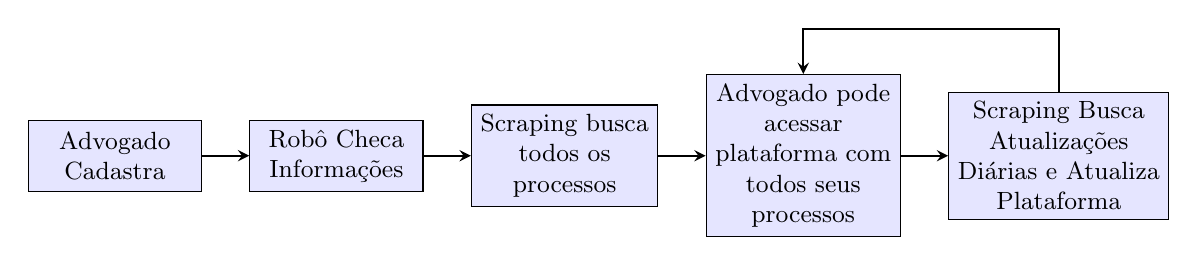
\begin{tikzpicture}[
    node distance=0.8cm,
    box/.style={rectangle, draw, minimum width=2.2cm, minimum height=0.9cm, align=center, fill=blue!10, font=\small},
    arrow/.style={->, >=stealth, thick}
]

\node[box] (cadastro) {Advogado\\Cadastra};
\node[box, right=0.6cm of cadastro] (valida) {Robô Checa\\Informações};
\node[box, right=0.6cm of valida] (busca) {Scraping busca\\todos os\\processos};
\node[box, right=0.6cm of busca] (acesso) {Advogado pode\\acessar\\plataforma com\\todos seus\\processos};
\node[box, right=0.6cm of acesso] (atualiza) {Scraping Busca\\Atualizações\\Diárias e Atualiza\\Plataforma};

\draw[arrow] (cadastro) -- (valida);
\draw[arrow] (valida) -- (busca);
\draw[arrow] (busca) -- (acesso);
\draw[arrow] (acesso) -- (atualiza);
\draw[arrow] (atualiza.north) -- ++(0,0.8) -| (acesso.north);

\end{tikzpicture}
	\end{center}
	\legend{Fonte: Elaboração Própria}
\end{figure}

\section{Relação das Atividades com as Disciplinas da Graduação}

As atividades desenvolvidas ao longo do estágio apresentaram relação direta com diversas disciplinas cursadas durante a graduação em Engenharia de Computação, permitindo a aplicação prática dos conhecimentos teóricos adquiridos.

A disciplina de \textbf{Banco de Dados} teve aplicação evidente em todo o projeto. A modelagem das entidades, a definição de índices adequados e a elaboração de consultas eficientes derivaram diretamente do conteúdo estudado. Em ambiente de produção, com volumes expressivos de dados, a importância de uma modelagem bem fundamentada tornou-se ainda mais clara, uma vez que consultas mal otimizadas impactavam diretamente o desempenho do sistema.

Os conceitos de \textbf{Engenharia de Software} foram aplicados na organização e gestão do projeto. A equipe adotou práticas de desenvolvimento ágil, com sprints planejados, manutenção de backlog e revisão de código. Embora a implementação prática apresentasse variações em relação à teoria, os fundamentos sobre ciclo de vida de software e metodologias ágeis forneceram a base necessária para estruturar o fluxo de trabalho.

Os princípios de \textbf{Programação Orientada a Objetos} foram aplicados de forma expressiva no desenvolvimento do sistema de scraping. A arquitetura adotada, com uma classe base abstrata e implementações específicas para cada tribunal, exemplifica a aplicação de conceitos como herança e polimorfismo em um contexto real.

Os conhecimentos de \textbf{Redes de Computadores} mostraram-se fundamentais para a implementação do web scraping. A compreensão do protocolo HTTP, do funcionamento de cookies e do mecanismo de manutenção de sessões foi essencial para simular adequadamente o comportamento de um navegador ao interagir com os portais dos tribunais.

A experiência prática obtida durante o estágio evidenciou como os conhecimentos teóricos adquiridos nas disciplinas da graduação se complementam na construção de sistemas reais, reforçando a importância de uma formação sólida nos fundamentos da Engenharia de Computação.

% ----------------------------------------------------------
% Referências bibliográficas
% ----------------------------------------------------------
\bibliography{referencias}

\end{document}
